\chapter{Criptografía y Curvas Elípticas}

En este capítulo voy a introducir la teoría sobre criptografía y curvas elípticas necesaria para entender la base detrás de los criptosistemas usados en las aplicaciones de mensajería más populares.

\section{Objetivos de la criptografía}
En este apartado voy a describir los objetivos de un criptosistema y los posibles ataques que se le pueden hacer. Además realizaré una introducción a la criptografía simétrica y asimétrica y su uso en las aplicaciones de mensajería. Todo esto nos permitirá entender los distintos criptosistemas que desarrollaré después.
La información de este apartado ha sido obtenida de \cite{apuntesCriptografia} para los criptosistemas simétricos y \cite{angelRiosMateos} para los cifrados asimétricos.\\
Los principales objetivos que debe cumplir todos los criptosistemas son:
\begin{description}
	\item \textbf{Confidencialidad.} 
		 La información solo puede ser accesible por las entidades autorizadas. 
	\item \textbf{Integridad.} 
		La información no ha sido alterada en el envío.
	\item \textbf{Autenticidad.} 
		La información proviene de quién afirma haberla enviado.
	\item \textbf{No repudio.}  
		El emisario de una información no puede negar haber realizado tal envío.
\end{description}
Para hablar de los ataques supondremos que se sigue el principio de \emph{Kerckhoffs}, el cual establece que el adversario conoce todos los detalles del criptosistema excepto la clave empleada.\\
Los posibles ataques son:
\begin{description}
		\item \textbf{Criptograma.} El adversario conoce el criptograma, es decir, el mensaje cifrado o un fragmento de este.
		\item \textbf{Mensaje Conocido.} El atacante conoce parejas mensaje/criptograma cifradas con una misma clave.
		\item \textbf{Mensaje escogido.} El atacante puede generar criptogramas para mensajes de su elección. Una vez obtenidas dichas parejas, trata de averiguar el mensaje correspondiente a un criptograma desconocido.
		\item \textbf{Mensaje escogido-adaptativo.} El atacante no solo puede generar pareas mensaje/criptograma a su elección, sino que puede hacerlo tantas veces como quiera realizando los análisis que considere oportunos.
		\item \textbf{Criptograma escogido y escogido-adaptativo.} Similar a los anteriores pero partiendo del criptograma, teniendo acceso a descifrar los criptogramas que desee, inicialmente o a lo largo del proceso. Lo que se busca en este ataque es la clave.
\end{description}

Una vez vistos los objetivos que tienen que cumplir los criptosistemas y los posibles ataques de los que pueden ser objeto, voy a explicar el uso de los criptosistemas simétricos y asimétricos en las aplicaciones de mensajería.\\

\subsection{Criptosistemas simétricos y asimétricos en las aplicaciones de mensajería}
Los criptosistemas simétricos y asimétricos conforman un elemento fundamental en las aplicaciones de mensajería. Criptosistemas de ambas familias se usan de manera conjunta para garantizar la confidencialidad, integridad, autenticidad y no repudio de los mensajes.\\
Los criptosistemas simétricos son utilizados para cifrar los mensajes. Esto es debido a su velocidad de cifrado, su uso reducido de recursos y su mejor manejo de grandes cantidades de datos.
Tienen el defecto de que si la clave es interceptada, el criptosistema es vulnerado y se pierde tanto la confidencialidad como la autenticidad de los mensajes. 
Para evitar esto se suele complementar con métodos seguros para el intercambio de la clave como puede ser el \emph{intercambio de claves Diffie-Hellman}.\\
Los criptosistemas asimétricos son muy utilizados para la firma y autentificación de los mensajes, garantizando de esta manera la seguridad de la aplicación y se complementan con cifrados simétricos a la hora de cifrar los mensajes para garantizar de esta forma una eficiencia mucho mayor. Ya que uno de los principales problemas que tienen es su complejidad algorítmica a la hora de cifrar y descifrar los mensajes.\\

\subsection{Criptosistema simétrico}
Un criptosistema simétrico es un criptosistema en el cual se utiliza una sola clave para cifrar y descifrar un mensaje o es necesario conocer la clave secreta para desencriptar un mensaje. La importancia para garantizar la seguridad de los criptosistemas simétricos reside en el secreto de la clave, mientras que el conocer el algoritmo utilizado no es tan importante como medida de seguridad. Es decir, lo importante es que el atacante no conozca la clave, mientras que conozca el algoritmo usado no lo es tanto.\\
Un criptosistema simétrico está formado por:
\begin{itemize}
	\item $\mathcal{M}$ el conjunto de los mensajes, elementos candidatos a ser encriptados.
	\item $\mathcal{C}$ el conjunto de los criptogramas o mensajes obtenido después del proceso de encriptar.
	\item $\mathcal{K} \subseteq \mathcal{K}_p\times\mathcal{K}_s$ el espacio de las claves, elementos que se utilizan para encriptar y desencriptar los mensajes. 
\end{itemize}
Un criptosistema simétrico viene definido por dos aplicaciones
$$E:\mathcal{K}_p\times\mathcal{M}\rightarrow\mathcal{C},$$
$$\mathcal{D}:\mathcal{K}_s\times\mathcal{C}\rightarrow\mathcal{M}.$$
tales que para cualquier clave $k_p \in \mathcal{K}_p$, existe una clave $k_s$ de manera que dato cualquier mensaje $m \in \mathcal{M}$,
$$
\mathcal{D}(k_s,E(k_p,m))=m.
$$
Fijada la clave $k_p \in \mathcal{K}_p$ y su correspondiente $k_s \in \mathcal{K}_s$ se definen las funciones de cifrado y descifrado como:\\
\begin{aligned}
	\center
	&$E_{k_p}:\mathcal{M}\rightarrow\mathcal{C},$\\
	&$E_{k_p}(m)=E(k_p,m),$
\end{aligned}
\begin{aligned}
	\center
	&$D_{k_p}:\mathcal{C}\rightarrow\mathcal{M},$\\
	&$D_{k_s}(c)=D(k_s,c),$
\end{aligned}

\subsection{Criptosistema asimétrico}
Un criptosistema asimétrico es un criptosistema en el cual se utilizan dos claves, una para cifrar el mensaje y otra para descifrarlo. La clave para cifrar es la que se conoce como \emph{clave pública}, mientras que la que se utiliza para descifrar es la \emph{clave privada}. Estos criptosistemas surgieron para paliar la debilidad de los criptosistemas simétricos, que es que la clave que cifra y descifra se tiene que compartir, pudiendo esta ser interceptada.  
La seguridad de estos criptosistemas reside en que no se conozca la clave privada.\\
Un criptosistema asimétrico está formado por:
\begin{itemize}
	\item $\mathcal{M}$ es el conjunto de los mensajes.
	\item $\mathcal{C}$ es el conjunto de los criptogramas.
	\item Una función $P:\mathcal{K}' \rightarrow \mathcal{K}$, que nos permitirá generar la clave pública. De manera que para cualquier clave privada $k' \in \mathcal{K}'$ obtenemos la clave pública como $P(k')=k$ 
\end{itemize}
Un criptosistema asimétrico viene definido por dos aplicaciones:
$$E:\mathcal{K}\times\mathcal{M}\rightarrow\mathcal{C},$$
$$\mathcal{D}:\mathcal{K}'\times\mathcal{C}\rightarrow\mathcal{M},$$
y se definen las funciones de cifrado y descifrado como:\\
\begin{aligned}
	\center
	&$E_{k}:\mathcal{M}\rightarrow\mathcal{C},$\\
	&$E_{k}(m)=E(k,m),$
\end{aligned}
\begin{aligned}
	\center
	&$D_{k^{'}}:\mathcal{C}\rightarrow\mathcal{M},$\\
	&$D_{k'}(c)=D(k',c).$
\end{aligned}

Para que un criptosistema asimétrico sea seguro tenemos que garantizar:
\begin{itemize}
	\item $P$ es una función de dirección única, es decir, que dado un elemento de su imagen no se puede calcular su imagen inversa fácilmente.
	\item Para la mayoría de los $k \in \mathcal{K}$, la aplicación $E_k$ es de dirección única.
	\item $\mathcal{D}_{k'}$ se puede calcular en un periodo corto de tiempo si se conoce $k'$ y es imposible o el periodo es muy largo en caso de solo conocerse $k$.
\end{itemize}

\subsection{Cifrados de bloque}
A continuación voy a introducir los cifrados de bloque, ya que estos son fundamentales a la hora de cifrar los mensajes en las aplicaciones de mensajería debido a su eficiencia. El cifrado de bloque más utilizado actualmente es el cifrado \textbf{Rindael AES}. La información ha sido obtenida de \cite{apuntesCriptografia}.\\
Los cifrados de bloque son criptosistemas de clave simétrica en los que la longitud de los bloques y claves es fija.\\
Este criptosistema se define
$$
	E:\mathbb{B}^K\times\mathbb{B}^N\rightarrow \mathbb{B}^N,
$$
$$
	D:\mathbb{B}^K\times\mathbb{B}^N\rightarrow \mathbb{B}^N,
$$
donde N es el tamaño del bloque y K es el tamaño de la clave.\\
Los cifrados tienen distintos modos de operación los cuales dependen solo del tamaño del bloque. Estos modos permiten garantizar la confidencialidad de los mensajes, si bien, no garantizan su integridad. La información para describir los modos la he complementado con \cite{bloquenuevo}.\\ 
Los distintos modos usados en los cifrados de bloque son:\\
\begin{itemize}
	\item \textbf{Electronic CodeBook}\\
	Modo en el cual para una clave dada, se le asigna un bloque de texto fijo cifrado por cada bloque de texto plano. Los pasos que se siguen para encriptar y desencriptar son:
	\begin{itemize}
		\item \textbf{\emph{Cifrado ECB}}
		\begin{description}
			\item Dividimos m en $m_{[1]}\dots m_{[l]}$ con $m_{[i]} \in \mathbb{B}^N$
			\item Para $i\in \{1,\dots,l\}$ hacer
			\begin{description}
				\item $c_{[i]} = E_k(m_{[i]})$
			\end{description}
			\item Devolvemos $c_{[1]}\dots c_{[l]}$
		\end{description}

		\item \textbf{\emph{Descifrado ECB}}
		\begin{description}
			\item Dividimos c en $c_{[1]}\dots c_{[l]}$ con $c_{[i]} \in \mathbb{B}^N$
			\item Para $i\in\{1,\dots,l\}$ hacer
			\begin{description}
				\item $m_{[i]} = D_k(c_{[i]})$
			\end{description}
			\item Devolvemos $m_{[1]}\dots m_{[l]}$
		\end{description}
	\end{itemize}
\newpage
		\begin{figure}[htb]
			\centering
			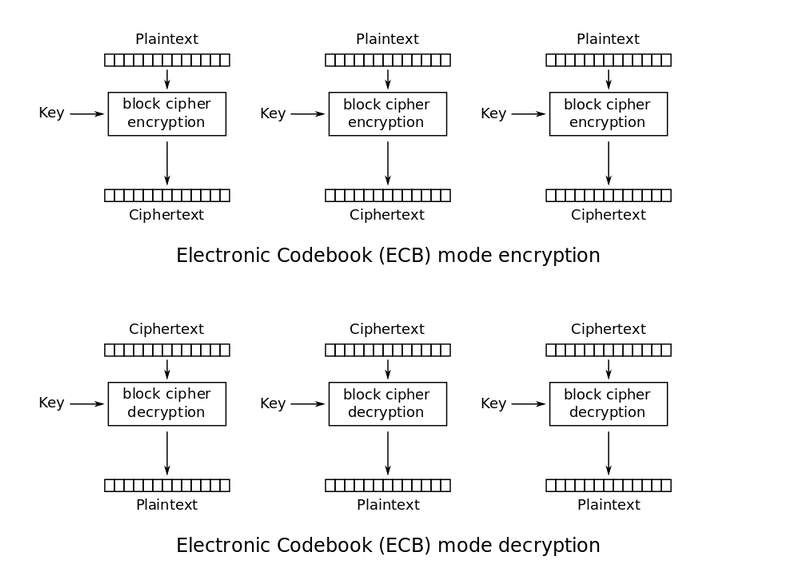
\includegraphics[scale=0.4]{imagenes/ecb.png} 
			\caption{Esquema del cifrado y descifrado del modo ECB \cite{cifradobloque}.}
			\label{esquemaecb}
		\end{figure}
		
	\item \textbf{Cipher-Block Chaining}\\
	En este modo se combina los bloques de texto plano con los bloques de texto cifrados anteriormente. Para cifrar el primer bloque será necesario un bloque inicial, $c_{[0]}$, el cual no tiene necesariamente que ser secreto. Los pasos seguidos para encriptar y desencriptar son:
	\begin{itemize}
		\item \textbf{\emph{Cifrado CBC}}
		\begin{description}
			\item $c_{[0]} \in \mathbb{B}^*$
			\item Dividimos m en $m_{[1]}\dots m_{[l]}$ con $m_{[i]} \in \mathbb{B}^N$
			\item Para $i\in\{1,\dots,l\}$ hacer
			\begin{description}
				\item $c_{[i]} = E_k(m_{[i]}\oplus c_{[i-1]})$
			\end{description}
			\item Devolvemos $c_{[1]}\dots c_{[l]}$
		\end{description}

		\item \textbf{\emph{Descifrado CBC}}
		\begin{description}
			\item Dividimos c en $c_{[0]}\dots c_{[l]}$ con $c_{[i]} \in \mathbb{B}^N$
			\item Para $i\in\{1,\dots,l\}$ hacer
			\begin{description}
				\item $m_{[i]} = D_k(c_{[i]})\oplus c_{[i]}$
			\end{description}
			\item Devolvemos $m_{[1]}\dots m_{[{l}]}$
		\end{description}
	\end{itemize}
\newpage
		\begin{figure}[htb]
			\centering
			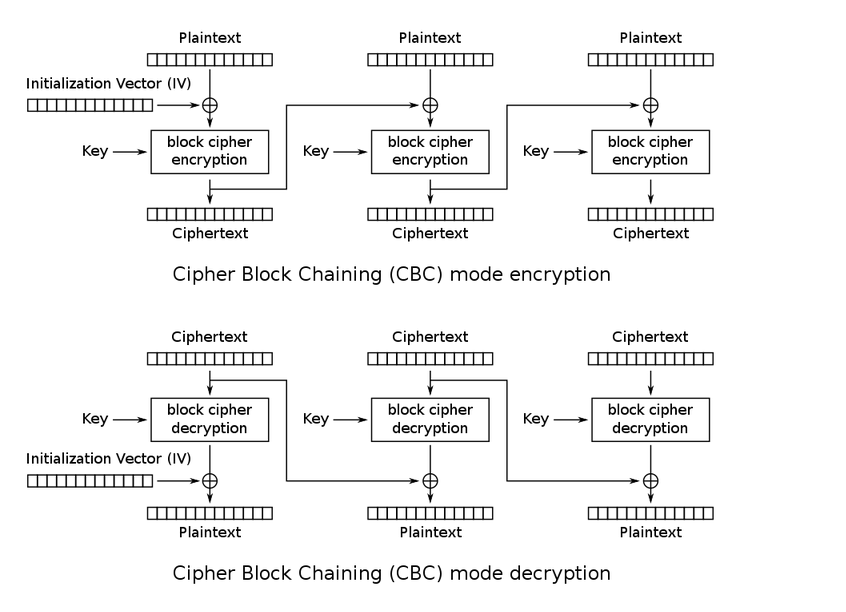
\includegraphics[scale=0.4]{imagenes/cbc.png} 
			\caption{Esquema del cifrado y descifrado del modo CBC \cite{cifradobloque}.}
			\label{esquemacbc}
		\end{figure}

	\item \textbf{Cipher FeedBack}\\
	Modo en el cual se combina cada bloque de texto plano del mensaje consigo mismo encriptado, los pasos que se siguen son:
	\begin{itemize}
		\item \textbf{\emph{Cifrado CFB}}
		\begin{description}
			\item $x_{[0]} \in \mathbb{B}^r$
			\item Dividimos m en $m_{[1]}\dots m_{[l]}$ con $m_{[i]} \in \mathbb{B}^N$
			\item Para $i\in\{1,\dots,l\}$ hacer
			\begin{description}
				\item $c_{[i]} = m_{[i]}\oplus msb_r(E_k(x_{[i]}))$
				\item $x_{[i+1]} = lsb_{N-r}(x_i)||c_{[i]$
			\end{description}
			\item Devolvemos $c_{[1]}\dots c_{[l]}$
		\end{description}

		\item \textbf{\emph{Descifrado CFB}}
		\begin{description}
			\item Dividimos c en $c_{[1]}\dots c_{[l]}$ con $c_{[i]} \in \mathbb{B}^r$
			\item Para $i\in\{1,\dots,l\}$ hacer
			\begin{description}
				\item $m_{[i]} = c_{[i]}\oplus msb_r(E_k(x_{[i]}))$
				\item $x_{[i+1]} = lsb_{N-r}(x_i)||c_{[i]$
			\end{description}
			\item Devolvemos $m_{[1]}\dots m_{[l]}$
		\end{description}
	\end{itemize}

%\newpage
		\begin{figure}[htb]
			\centering
			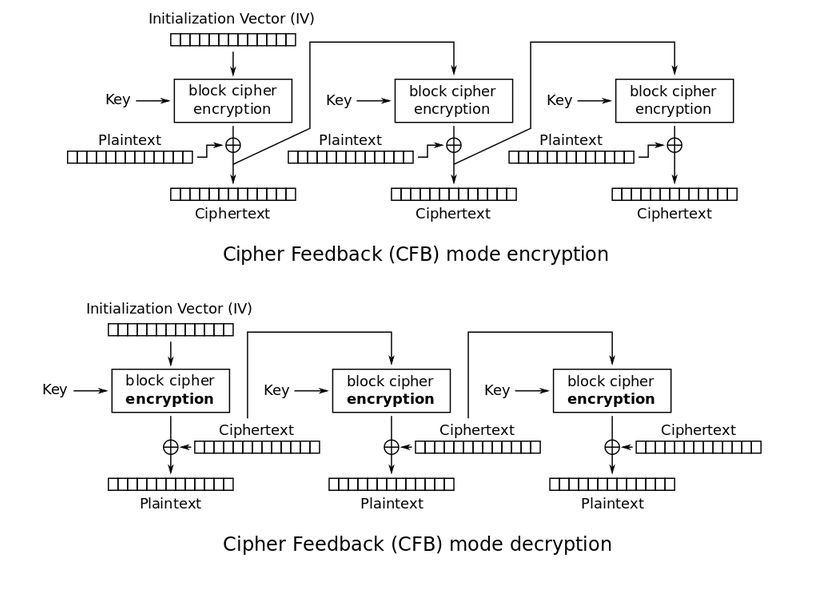
\includegraphics[scale=0.4]{imagenes/cfb.png} 
			\caption{Esquema del cifrado y descifrado del modo CFB \cite{cifradobloque}.}
			\label{esquemacfb}
		\end{figure}

\newpage
	\item \textbf{Output FeedBack}\\
	Modo en el cual se parte de un bloque inicial $x_{[0]}$ único y secreto. En cada iteración se encripta este y se combina con un bloque del mensaje sin cifrar de manera recursiva. Los pasos seguidos para encriptar y desencriptar son:
	\begin{itemize}
		\item \textbf{\emph{Cifrado OFB}}
		\begin{description}
			\item $x_{[0]} \in \mathbb{B}^N$
			\item Dividimos m en $m_{[1]}\dots m_{[l]}$ con $m_{[i]} \in \mathbb{B}^N$
			\item Para $i\in\{1,\dots,l\}$ hacer
			\begin{description}
				\item $x_{[i]} = E_k(x_{[i-1]})$
				\item $c_{[i]} = m_{[i]}\oplus x_{[i]}$
			\end{description}
			\item Devolvemos $c_{[1]}\dots c_{[l]}$
		\end{description}

		\item \textbf{\emph{Descifrado OFB}}
		\begin{description}
			\item Dividimos c en $c_{[1]}\dots c_{[l]}$ con $c_{[i]} \in \mathbb{B}^N$
			\item Para $i\in\{1,\dots,l\}$ hacer
			\begin{description}
				\item $x_{[i]} = E_k(x_{[i-1]})$
				\item $m_{[i]} = c_{[i]}\oplus x_{[i]}$
			\end{description}
			\item Devolvemos $m_{[1]}\dots m_{[l]}$
		\end{description}
	\end{itemize}
		\begin{figure}[htb]
			\centering
			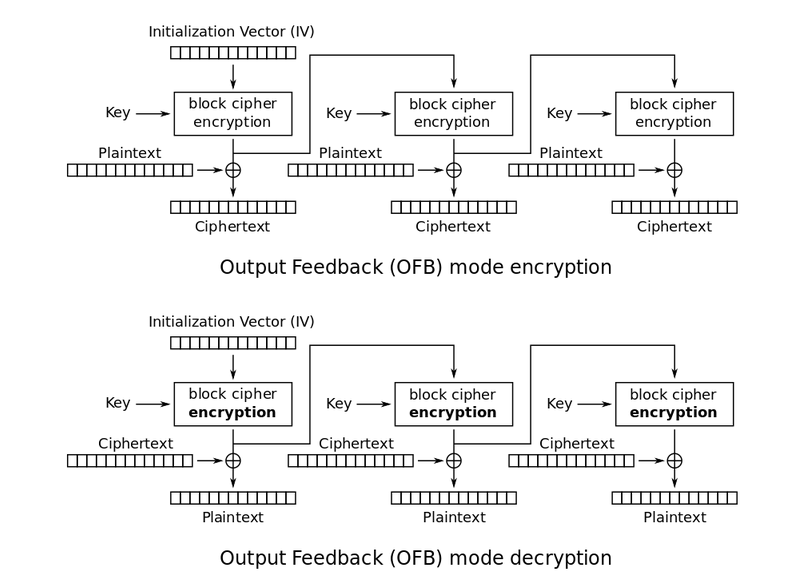
\includegraphics[scale=0.4]{imagenes/ofb.png} 
			\caption{Esquema del cifrado y descifrado del modo OFB \cite{cifradobloque}.}
			\label{esquemaofb}
		\end{figure}
\end{itemize}
\newpage
Como podemos ver, el más sencillo es ECB ya que lo único que hace es fragmentar el mensaje en bloques y encriptar individualmente cada bloque. En CBC, CFB y OFB se parte de un bloque inicial y se generan bloques nuevos de manera recursiva operando con ellos de manera distinta en función de cada modo.\\ 
En CBC se realiza la operación $\oplus$ de cada bloque generado encriptándose el bloque cifrado previo a esta con un bloque del mensaje, los nuevos bloques son los resultados de la operación anterior.\\
En CFB se coge el bit menos significativo resultante de encriptar el bloque generado previo y se hace la operación $\oplus$ con cada bloque del mensaje. Para generar un nuevo bloque se combina el mensaje cifrado previo con el bit menos significativo del conjunto de bits $N-r$ del bloque generado anterior con la operación $||$.\\
Y en OFB se realiza la operación $\oplus$ de el resultado de encriptar el bloque generado previo con un bloque del mensaje.\\
Actualmente el más utilizado en las aplicaciones de mensajería es el modo CBC. Esto es debido a que es relativamente fácil de implementar y además permite encriptar en paralelo.

\section{El algoritmo Rijndael AES}
En esta sección explicaré el cifrado Rijndael AES el cual es un cifrado de bloque simétrico muy utilizado actualmente por aplicaciones como \emph{Telegram}, \emph{WhatsApp} y \emph{FacebookChat} entre otras.\\
El algoritmo Rijndael llamado así en honor a sus dos autores Joan Daemen y Vicent Rijmen, es un algoritmo de cifrado por bloques que fue adoptado en octubre de 2000 por el NIST (\emph{National Institute for Standards and Technology}) para su empleo en aplicaciones criptográficas no militares en sustitución del algoritmo \emph{DES} después de un proceso de más tres años en los que se buscaba un algoritmo que fuera potente, eficiente y fácil de implementar.\\
Está diseñado para manejar longitudes de clave y de bloque variables entre los 128 y los 256 bits y aunque estos sean variables, en el estándar adoptado por el Gobierno de Estados Unidos en 2001 \cite{aesUsa} establece una longitud fija de bloque de 128 bits y una longitud de clave a escoger entre 128, 192 y 256 bits.\\
La información para los siguientes apartados de AES la he obtenido de \cite{En2011} y de \cite{criptografia}.\\

\subsection{Estructura de AES}
AES es un algoritmo que se basa en aplicar un número determinado de rondas a un valor intermedio denominado \emph{estado} que puede ser representado por una matriz rectangular que posee cuatro filas y $N_{b}$ columnas. Análogamente, la clave tiene la misma estructura, una matriz de cuatro filas y $N_{k}$ columnas.
El bloque a cifrar o descifrar se traslada directamente byte a byte sobre la matriz de estado de columna en columna ($a_{0,0}, a_{1,0}, a_{2,0}, a_{3,0}, a_{0,1} \dots$).

\begin{table}[htb]
	\begin{center}
		\begin{tabular}{| l | l | l | l |}
				\hline
				$\math{a}_{0,0}$ & $\math{a}_{0,1}$ & $\math{a}_{0,2}$ & $\math{a}_{0,3}$\\ \hline
				$\math{a}_{1,0}$ & $\math{a}_{1,1}$ & $\math{a}_{1,2}$ & $\math{a}_{1,3}$\\ \hline
				$\math{a}_{2,0}$ & $\math{a}_{2,1}$ & $\math{a}_{2,2}$ & $\math{a}_{2,3}$\\ \hline
				$\math{a}_{3,0}$ & $\math{a}_{3,1}$ & $\math{a}_{3,2}$ & $\math{a}_{3,3}$\\ \hline
		\end{tabular}
		\caption{Ejemplo de matriz de estado con $N_b=4$(128 bits).}
	\end{center}
\end{table}

\begin{table}[htb]
	\begin{center}
		\begin{tabular}{| l | l | l | l |}
				\hline
				$\math{k}_{0,0}$ & $\math{k}_{0,1}$ & $\math{k}_{0,2}$ & $\math{k}_{0,3}$\\ \hline
				$\math{k}_{1,0}$ & $\math{k}_{1,1}$ & $\math{k}_{1,2}$ & $\math{k}_{1,3}$\\ \hline
				$\math{k}_{2,0}$ & $\math{k}_{2,1}$ & $\math{k}_{2,2}$ & $\math{k}_{2,3}$\\ \hline
				$\math{k}_{3,0}$ & $\math{k}_{3,1}$ & $\math{k}_{3,2}$ & $\math{k}_{3,3}$\\ \hline
		\end{tabular}
		\caption{Ejemplo de clave con $N_k=4$(128 bits).}
	\end{center}
\end{table}

En otros casos el bloque y la clave pueden ser representados como vectores de registro de 32 bits, donde cada registro esta compuesto por los bytes de la columna correspondiente ordenados en orden descendiente.\\

Siendo $B$ el bloque que queremos cifrar y $S$ la matriz de estado, el algoritmo AES con $n$ rondas se resume en:

\begin{enumerate}
	\item Calcular $K_0, K_1,...,K_n$ subclaves a partar de la clave $K$.
	\item $S\leftarrow B \oplus K_0$.
	\item Para $i=1$ hasta $n$ hacer:
	\begin{description}
			\item Aplicar la ronda \emph{i}-ésima del algoritmo con la subclave $K_i$.
	\end{description}
\end{enumerate}
Como las funciones usadas en cada ronda son invertibles, para descifrar aplicaremos las funciones inversas de las funciones usadas para cifrar en el orden opuesto.

\begin{table}[htb]
	\begin{center}
		\begin{tabular}{| l | l | l | l |}
				\hline
				& $N_b = 4$(128 bits) & $N_b = 6$(192 bits)& $N_b = 8$(256 bits)\\ \hline
				$N_k = 4$(128 bits)& 10 & 12 & 14\\ \hline
				$N_k = 6$(128 bits)& 12 & 12 & 14\\ \hline
				$N_k = 8$(128 bits)& 14 & 14 & 14\\ \hline
		\end{tabular}
		\caption{Número de rondas en función del tamaño de la clave y bloque.}
		\label{rondas_aes}
	\end{center}
\end{table}


En el algoritmo AES se define cada ronda como una composición de cuatro funciones invertibles diferentes, formando tres \emph{capas}. Estas funciones tienen un propósito específico.
\begin{itemize}
	\item \textbf{Capa de mezcla lineal:} formada por las funciones \emph{DesplazarFila} y \emph{MezclarColumnas} que permite obtener un alto nivel de difusión a lo largo de varias rondas.
	\item \textbf{Capa no lineal:} formada por la función \emph{ByteSub} y es la aplicación paralela de s-cajas con propiedades óptimas de no linealidad.
	\item \textbf{Capa de adición de clave:} es un simple \emph{o-exclusivo} entre el estado intermedio y la subclave correspondiente a cada ronda.
\end{itemize}

\subsection{El cuerpo de Galois $\operatorname{GF}(2^n)$}
Tanto para explicar el funcionamiento de las rondas de AES como para desarrollar la teoría de Curvas Elípticas en $\operatorname{GF}(2^n)$ es necesario introducir el cuerpo $\operatorname{GF}(2^n)$. El cual debido a las propiedades que tiene es muy utilizado en criptografía.\\
Sea $\mathbb{Z}_2[x]$ el conjunto de polinomios con coeficientes en $\mathbb{Z}_2$, es decir, el conjunto de polinomios cuyos coeficientes solo valen 0 ó 1. Así los polinomios pueden ser representados por una cadena de bits.
 Un ejemplo sería el polinomio $f(x)=x^4+x^3+x+1$ que quedaría representado como 11011. 
Además si lo sumamos con otro polinomio como puede ser $g(x)=x^2+x+1$, tenemos que $f(x)+g(x)=x^4+x^3+x^2$, que equivale a hacer la operación XOR entre 11011 y 00111, por lo que a nivel computacional, es muy fácil implementar estas operaciones.\\
Podemos definir el cuerpo $\operatorname{GF}(2^n)$ como $\mathbb{Z}_2[x]/(a(x))$, con $a(x)$ un polinomio irreducible en $\mathbb{Z}/(a(x))$. Tenemos que la existencia del inverso de cualquier polinomio no nulo está asegurada por el algoritmo Extendido de Euclídes.\\ 
Principalmente se trabaja con $\operatorname{GF}(2^n)$ debido a que la implementación de las operaciones de este es más sencilla que la implementación en las que se utilizan otros cuerpos. Ya que como hemos visto, es muy fácil implementar las operaciones. Por lo que teniendo el mismo orden de complejidad, se multiplica la velocidad permitiendo obtener sistemas con mejores prestaciones.\\
A continuación presentaré el cuerpo $\operatorname{GF}(2^8)$ ya que será necesario para entender adecuadamente las operaciones utilizadas en AES. La información ha sido obtenida de \cite{criptografia} y \cite{dem1}.\\
Tenemos que $\operatorname{GF}(2^8)=\mathbb{F}_{256}$ por lo que por comodidad trabajaremos con este último.\\
Por definición tenemos que para $p$ número primo y $n$ se define el cuerpo $\mathbb{F}_{p^n}$ al único cuerpo existente con $p^n$ elementos. En particular para trabajar con $\mathbb{F}_{256}$ tomamos $p=2$ y $n=8$.\\
Para construir $\mathbb{F}_{256}$ necesitamos un polinomio de grado 8, con coeficientes en $\mathbb{Z}_2$ y que sea irreducible. En total hay 30 polinomios con esas características donde algunos de ellos son 
$x^8+x^4+x^3+x+1$, $\:x^8+x^4+x^3+x^2+1$, $x^8+x^5+x^3+x+1$, $x^8+x^5+x^3+x^2+1$, $x^8+x^5+x^4+x^3+1$, $x^8+x^5+x^4+x^3+x^2+x+1$ y $x^8+x^6+x^3+x^2+1$.\\ 
Cabe a destacar que cualquiera de los polinomios serviría para definir $\mathbb{F}_{256}$ y además no habría ninguna diferencia en la seguridad en los criptosistemas que lo utilicen. 
Para AES se tomó el polinomio $x^8+x^4+x^3+x+1$, por lo que a partir de ahora trabajaremos con $\mathbb{Z}_{2_{x^8+x^4+x^3+x+1}}[x]$.\\
Los elementos que conformarán al cuerpo serán clases de equivalencia de polinomios  de grado menor que 8. Cada elemento podrá ser representado de tres formas distintas además de la forma polinomial, como número binario, número hexadecimal y número decimal. Por ejemplo el polinomio $x^5+x+1$ quedaría representado como $00100011$ de manera decimal, $23$ en hexadecimal y $35$ en decimal.\\
Al ser $\mathbb{F}_{256}$ un cuerpo tenemos que tiene dos operaciones, la operación suma que representaremos como $+$ y la operación producto que representaremos como $\cdot$.\\
La operación $+$ equivale a la suma en $\mathbb{Z}_2$ y usando la notación en binario, tendríamos que equivaldría con la operación XOR como ya he mencionado anteriormente. El opuesto para la suma de un elemento equivalente a sí mismo por lo que no habría diferencia entre sumar por un número o por su apuesto, luego tendríamos que la suma es la misma operación que la resta.\\
La operación $\cdot$  es mucho más compleja ya que en principio habría que realizar la operación en notación polinomial y luego calcular el resto de dividir por $x^8+x^4+x^3+x+1$. Para calcular el inverso tendríamos que utilizar el algoritmo extendido de Euclídes. Ambos algoritmos tienen una complejidad algorítmica importante, pero se puede reducir. A continuación desarrollaré unos resultados de cuerpos finitos que nos permitirá obtener unos métodos que reducirán mucho esa complejidad.\\
\begin{definicion}
	Sea $K=\mathbb{F}_q$ un cuerpo finito $(q=p^n)$. Un elemento primitivo de $K$ es un elemento $\alpha$ que tiene $q-1$ potencias distintas.
\end{definicion}

\begin{teorema}
	(Teorema Fundamental de los Grupos Abelianos) Todo grupo abeliano finito $G$ es isomorfo a un producto directo de grupo cíclicos de la forma
	$$
		\mathbb{Z}_{p^{\alpha_1}_1}\times \dots \times \mathbb{Z}_{p^{\alpha_n}_n},
	$$
	donde los $p_i$ son primos no necesariamente diferentes.
\end{teorema}

\begin{teorema}
		Si $G$ es un subgrupo finito de $F^*$, el grupo multiplicativo de elementos no nulos de un cuerpo $F$, entonces $G$ es cíclico.
\end{teorema}\vspace*{-7mm}
\begin{proof}
		Sea $G$ un subgrupo finito de $F^*$ de orden $n$. Por el Teorema Fundamental de Grupos Abelianos tenemos,
		$$
			G \cong \mathbb{Z}_{p^{e_1}_1}\times \dots \times \mathbb{Z}_{p^{e_k}_k},
		$$
		donde $n = p^{e_1}_1 \dots p^{e_k}_k$ y los $p_1, \dots, p_k$ son primos no necesariamente distintos. Sea $m$ el mínimo común múltiplo de $p^{e_1}_1 \dots p^{e_k}_k$. Entonces $G$ contiene un elemento de orden $m$. Como todo $\alpha$ en $G$ satisface $x^r-1$ para algún $r$ que divide a $m$, $\alpha$ debe también ser raíz de $x^m-1$. Como $x^m-1$ tienen a lo más $m$ raíces en $F$, $n\leq m$. Por otra parte, sabemos que $m\leq |G|$, por lo tanto, $m=n$. Luego $G$ contiene un elemento de orden $n$ y tiene que ser cíclico.\qedhere
\end{proof}

\begin{corolario}
		El grupo multiplicativo de todos los elementos no nulos de un cuerpo finito es cíclico.
\end{corolario}

Por lo que si $\alpha$ es un elemento primitivo de $\mathbb{F}_q$, los $q-1$ elementos de la forma\\
$$
	\alpha^0=1,\;\; \alpha^1=\alpha,\;\dots\; ,\alpha^{q-2}
$$
serán todos independientes, es decir, distintos y no nulos. Por tanto serán todos los elementos no nulos de $\mathbb{F}_q$. Además, se verifica que $\alpha^{q-1}=\alpha^0$ por lo que para cualquier $n \in \mathbb{Z}$ se cumple que $\alpha^n=\alpha^{n\mod q-1}$.\\

\begin{teorema}
	Todo cuerpo finito tiene al menos un elemento primitivo.
\end{teorema}
Salvo para $q=2$, el número de elementos primitivos de $\mathbb{F}_q$ es $\phi(q-1)$. Para el caso $q=13$ se tiene que $\phi(12)=\phi(2^2\cdot 3)=2\cdot2=4$, luego $\mathbb{Z}_{13}$ tiene 4 elementos primitivos que son 2, 6, 7 y 11. En $\mathbb{F}_{256}$ tenemos que hay $\phi(256)=128$ elementos primitivos.

Ahora para multiplicar dos elementos pertenecientes a $\mathbb{Z}_{13}$ podemos usar su logaritmo en base 2, el exponente que hay que elevar 2 para obtener el número, sumar los logaritmos y reducirlos base 13 y elevar 2 al resultado. Un ejemplo sería:
$$
	10\cdot12=2^{10}\cdot2^{6}=2^{16}=2^3=8.
$$
Para calcular el inverso sería:
$$
	12^{-1}=(2^6)^{-1}=2^{12-6}=2^6=12.
$$
Esta es la idea que nos permite optimizar las multiplicaciones y los cálculos de inversos en $\mathbb{F}_{256}$. Para ello elegimos un elemento primitivo que nos servirá de generador, en este caso nosotros utilizaremos el más pequeño, que es $[x+1]$ en notación polinomial, 00000011 en binario, 03 en hexadecimal y 3 en binario. Por comodidad trabajaremos en hexadecimal. 

\begin{table}[!htb]
    %\begin{adjustwidth}{-.8in}{-.8in}  
\resizebox{\textwidth}{!}{%
\begin{tabular}{|l|l|l|l|l|l|l|l|l|l|l|l|l|l|l|l|l|}
\hline
\multicolumn{1}{|r|}{} & 0  & 1  & 2  & 3  & 4  & 5  & 6  & 7  & 8  & 9  & A  & B  & C  & D  & E  & F  \\ \hline
0                      & 01 & 03 & 05 & 0F & 11 & 33 & 55 & FF & 1A & 2E & 72 & 96 & A1 & F8 & 13 & 35 \\ \hline
1                      & 5F & E1 & 38 & 48 & D8 & 73 & 95 & A4 & F7 & 02 & 06 & 0A & 1E & 22 & 66 & AA \\ \hline
2                      & E5 & 34 & 5C & E4 & 37 & 59 & EB & 26 & 6A & BE & D9 & 70 & 90 & AB & E6 & 31 \\ \hline
3                      & 53 & F5 & 04 & 0C & 14 & 3C & 44 & CC & 4F & D1 & 68 & B8 & D3 & 6E & B2 & CD \\ \hline
4                      & 4C & D4 & 67 & A9 & E0 & 3B & 4D & D7 & 62 & A6 & F1 & 08 & 18 & 28 & 78 & 88 \\ \hline
5                      & 83 & 9E & B9 & D0 & 6B & BD & DC & 7F & 81 & 98 & B3 & CE & 49 & DB & 76 & 9A \\ \hline
6                      & B5 & C4 & 57 & F9 & 10 & 30 & 50 & F0 & 0B & 1D & 27 & 69 & BB & D6 & 61 & A3 \\ \hline
7                      & FE & 19 & 2B & 7D & 87 & 92 & AD & EC & 2F & 71 & 93 & AE & E9 & 20 & 60 & A0 \\ \hline
8                      & FB & 16 & 3A & 4E & D2 & 6D & B7 & C2 & 5D & E7 & 32 & 56 & FA & 15 & 3F & 41 \\ \hline
9                      & C3 & 5E & E2 & 3D & 47 & C9 & 40 & C0 & 5B & ED & 2C & 74 & 9C & BF & DA & 75 \\ \hline
A                      & 9F & BA & D5 & 64 & AC & EF & 2A & 7E & 82 & 9D & BC & DF & 7A & 8E & 89 & 80 \\ \hline
B                      & 9B & B6 & C1 & 58 & E8 & 23 & 65 & AF & EA & 25 & 6F & B1 & C8 & 43 & C5 & 54 \\ \hline
C                      & FC & 1F & 21 & 63 & A5 & F4 & 07 & 09 & 1B & 2D & 77 & 99 & B0 & CB & 46 & CA \\ \hline
D                      & 45 & CF & 4A & DE & 79 & 8B & 86 & 91 & A8 & E3 & 3E & 42 & C6 & 51 & F3 & 0E \\ \hline
E                      & 12 & 36 & 5A & EE & 29 & 7B & 8D & 8C & 8F & 8A & 85 & 94 & A7 & F2 & 0D & 17 \\ \hline
F                      & 39 & 4B & DD & 7C & 84 & 97 & A2 & FD & 1C & 24 & 6C & B4 & C7 & 52 & F6 & 01 \\ \hline
\end{tabular}}
	\label{antilogaritmos}
	%\end{adjustwidth}
\caption{Tabla de los antilogaritmos de $[x+1]$}
\end{table}
Por ejemplo para calcular el resultado de $[x+1]^{125}=(03)^{125}$ lo que hacemos es escribir 125 en hexadecimal que es 7D. A continuación miramos en la tabla, la fila 7 y la columna D que nos da 20 luego tendríamos que $(03)^{125}=20$. Pasándolo a forma polinomial tenemos que $[x+1]^{125}=x^5$.\\
Para construir la tabla es mejor usar la forma binaria.\\

A continuación vamos a construir la tabla inversa de la anterior, esta nos permitirá calcular dado un $z \in \mathbb{F}_{256}$ con $z \neq 0$ el valor de $y$ que verifica $[x+1]^y=z$ que denominaremos $\log_{x+1}(z)$.
\begin{table}[!htb]
    %\begin{adjustwidth}{-.8in}{-.8in}  
\resizebox{\textwidth}{!}{%
\begin{tabular}{|l|l|l|l|l|l|l|l|l|l|l|l|l|l|l|l|l|}
\hline
  & 0  & 1  & 2  & 3  & 4  & 5  & 6  & 7  & 8  & 9  & A  & B  & C  & D  & E  & F  \\ \hline
0 &    & 00 & 19 & 01 & 32 & 02 & 1A & C6 & 4B & C7 & 1B & 68 & 33 & EE & DF & 03 \\ \hline
1 & 64 & 04 & E0 & 0E & 34 & 8D & 81 & EF & 4C & 71 & 08 & C8 & F8 & 69 & 1C & C1 \\ \hline
2 & 7D & C2 & 1D & B5 & F9 & B9 & 27 & 6A & 4D & E4 & A6 & 72 & 9A & C9 & 09 & 78 \\ \hline
3 & 65 & 2F & 8A & 05 & 21 & 0F & E1 & 24 & 12 & F0 & 82 & 45 & 35 & 93 & DA & 6E \\ \hline
4 & 96 & 8F & DB & BD & 36 & D0 & CE & 94 & 13 & 5C & D2 & F1 & 40 & 46 & 83 & 38 \\ \hline
5 & 66 & DD & FD & 30 & BF & 06 & 8B & 62 & B3 & 25 & E2 & 98 & 22 & 88 & 91 & 10 \\ \hline
6 & 7E & 6E & 48 & C3 & A3 & B6 & 1E & 42 & 3A & 6B & 28 & 54 & FA & 85 & 3D & BA \\ \hline
7 & 2B & 79 & 0A & 15 & 9B & 9F & 5E & CA & 4E & D4 & AC & E5 & F3 & 73 & A7 & 57 \\ \hline
8 & AF & 58 & A8 & 50 & F4 & EA & D6 & 74 & 4F & AE & E9 & D5 & E7 & E6 & AD & E8 \\ \hline
9 & 2C & D7 & 75 & 7A & EB & 16 & 0B & F5 & 59 & CB & 5F & B0 & 9C & A9 & 51 & A0 \\ \hline
A & 7F & 0C & F6 & 6F & 17 & 74 & 49 & EC & D8 & 43 & 1F & 2D & A4 & 76 & 7B & B7 \\ \hline
B & CC & BB & 3E & 5A & FB & 60 & B1 & 86 & 3B & 52 & A1 & BC & AA & 55 & 29 & 9D \\ \hline
C & 97 & B2 & 87 & 90 & 61 & BE & DC & FC & B5 & 95 & CF & CD & 37 & 3F & 5B & D1 \\ \hline
D & 53 & 39 & 84 & 3C & 41 & A2 & 6D & 47 & 14 & 2A & 9E & 5D & 56 & F2 & D3 & AB \\ \hline
E & 44 & 11 & 92 & D9 & 23 & 20 & 2D & 89 & B4 & 7C & B8 & 26 & 77 & 99 & E3 & A5 \\ \hline
F & 67 & 48 & ED & DE & C5 & 31 & FE & 18 & 0D & 63 & 8C & 80 & C0 & F7 & 70 & 07 \\ \hline
\end{tabular}}
	\label{potenciasinversas}
    %\end{adjustwidth}
\caption{Tabla de los logaritmos de $[x+1]$}
\end{table}
\newpage
A partir de estas dos tablas ya podemos hacer sin mucha dificultad a nivel computacional multiplicaciones y cálculo de inversos. En general para realizar el producto de dos elementos $X$ e $Y$ lo haremos de la siguiente manera:
$$
	X\cdot Y = A\log((\log_{x+1}(X)+log_{x+1}(Y)) \mod 255).
$$
Donde $A\log$ es el antilogaritmo.\\
Análogamente para calcular el inverso tenemos:
$$
	X^{-1} = A\log(FF-\log_{x+1}(X)).
$$

Por ejemplo para calcular $[x^7+x^6+x^4+x^2+x]\cdot[x^6+x^5+x^4+x^2+1]$ hacemos lo siguiente:
\begin{enumerate}
	\item Pasamos ambos polinomios a la forma hexadecimal como hemos visto anteriormente, en este caso nos quedaría $D6$ y $75$.
	\item Nos vamos a la tabla de logaritmos y obtenemos que $\log_{03}(D6)=6D$ y $\log_{03}(75)=9F$.
	\item Sumamos ambos resultados y lo reducimos módulo $255$, parar ello lo pasamos a decimal por comodidad $(109+159)\mod255=13$.
	\item Calculamos el antilogaritmo de $13=0D$ con la tabla y tenemos que vale $F8$ por lo que tenemos que $D6\cdot 75 = F8$.
\end{enumerate}

%\newpage
\subsection{Las Rondas de AES}
Una vez visto algunas de las propiedades de los cuerpos finitos, ya disponemos de las herramientas necesarias para describir las rondas de AES.
Dado que este algoritmo puede aplicarse para longitudes diferentes de bloque y clave, el número de rondas es variable, como se ha visto en \ref{rondas_aes}.\\
Siendo $S$ la matriz de estado y $K_i$ la subclave correspondiente a la ronda $i$-ésima, cada ronda posee esta estructura:
\begin{enumerate}
	\item $S \leftarrow ByteSub(S)$,
	\item $S \leftarrow DesplazarFila(S)$,
	\item $S \leftarrow MezclarColumnas(S)$,
	\item $S \leftarrow K_i \oplus S$.
\end{enumerate}
En la última ronda se hacen solo los tres primeros pasos del algoritmo.

	\subsubsection{ByteSub}
		La función \emph{ByteSub} es una sustitución no lineal que se aplica a cada byte de la matriz de estado mediante una s-caja 8\texttimes8. Se obtiene componiendo dos transformaciones:
		\begin{enumerate}
			\item Cada byte se considera como un elemento del $\operatorname{GF}(2^8)$ generado por el polinomio irreducible $m(x)=x^8+x^4+x^3+x+1$ y es sustituido por su inversa multiplicativa quedando el valor cero inalterado. 
			\item A continuación se aplica la siguiente transformación afín en $\operatorname{GF}(2)$ siendo $x_0, x_1,...,x_7$ los bits del byte correspondiente e $y_0, y_1,...,y_7$ los del resultado:

				\begin{equation*} 
					\begin{bmatrix} 
						y_0\\
						y_1\\
						y_2\\
						y_3\\
						y_4\\
						y_5\\
						y_6\\
						y_7\\
					\end{bmatrix}
					=
					\begin{bmatrix} % O matrices como esta de 4 x 3
						1 & 0 & 0 & 0 & 1 & 1 & 1 & 1\\
						1 & 1 & 0 & 0 & 0 & 1 & 1 & 1\\
						1 & 1 & 1 & 0 & 0 & 0 & 1 & 1\\
						1 & 1 & 1 & 1 & 0 & 0 & 0 & 1\\
						1 & 1 & 1 & 1 & 1 & 0 & 0 & 0\\
						0 & 1 & 1 & 1 & 1 & 1 & 0 & 0\\
						0 & 0 & 1 & 1 & 1 & 1 & 1 & 0\\
						0 & 0 & 0 & 1 & 1 & 1 & 1 & 1\\
					\end{bmatrix}
					\begin{bmatrix}
						x_0\\
						x_1\\
						x_2\\
						x_3\\
						x_4\\
						x_5\\
						x_6\\
						x_7\\
					\end{bmatrix}
					+
					\begin{bmatrix}
						1\\
						1\\
						0\\
						0\\
						0\\
						1\\
						1\\
						0\\
					\end{bmatrix}
			\end{equation*}
		\end{enumerate}
		La función inversa de $ByteSub$ es la aplicación inversa de la s-caja de cada byte de la matriz de estado.

	\subsubsection{DesplazarFila}
		Esta función desplaza a la izquierda de manera cíclica las filas de la matriz de estado. Cada fila $f_i$ se desplaza un número de posiciones $c_i$ diferente. Mientras que $c_0$ siempre es igual a cero, el resto de valores vine en función de $N_b$ como se puede ver en \ref{ciennb}.\\
		La función inversa será el desplazamiento de las filas de la matriz el mismo número de posiciones pero en el sentido contrario.

		\begin{table}[htb]
			\begin{center}
				\begin{tabular}{| l | l | l | l |}
						\hline
						$N_b$ & $c_1$ & $c_2$ & $c_3$\\ \hline
						4 & 1 & 2 & 3\\ \hline 
						6 & 1 & 2 & 3\\ \hline 
						8 & 1 & 3 & 4\\ \hline 
				\end{tabular}
				\caption{Valores de $c_i$ según el tamaño de bloque $N_b$}
				\label{ciennb}
			\end{center}
		\end{table}

		\begin{figure}[htb]
			\centering
			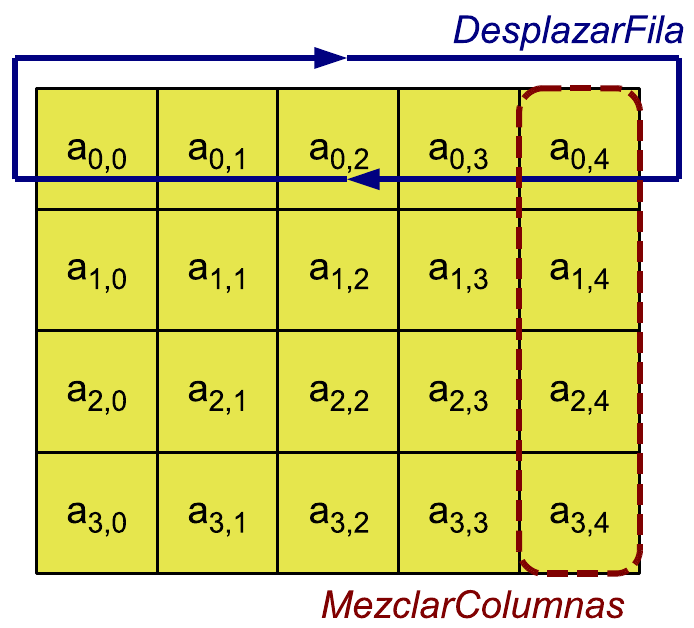
\includegraphics[scale=0.4]{imagenes/aesdesplazarmezclar.png} 
			\caption{Esquema de las funciones $MezclarColumnas$ y $DesplazarFila$ \cite{En2011}}
			\label{desplazarymezclar}
		\end{figure}
%\newpage
	\subsubsection{MezclarColumnas}
	Durante la aplicación de esta función cada columna del vector de estado es vista como una matriz $4 \times 1$ donde sus coeficientes pertenecen a $\mathbb{F}_{256}$. Aplicar MezclarColumnas a cada estado equivale a multiplicar cada columna por la matriz $4 \times 4$.

			\begin{center}
					\begin{pmatrix} 
						02 & 03 & 01 & 01 \\
						01 & 02 & 03 & 01 \\
						01 & 01 & 02 & 03 \\
						03 & 01 & 01 & 02 \\
					\end{pmatrix}
			\end{center}

\subsection{Cálculo de las Subclaves}
Las subclaves $K_i$ se obtienen de la clave principal $K$ mediante el uso de dos funciones: una de expansión y otra de selección. Siendo $n$ el número de rondas que se van a aplicar, la función de expansión obtiene a partir del valor de $K$ una secuencia de $4(n+1)N_b$ bytes.\\
La función de selección toma consecutivamente de la secuencia obtenida bloques del mismo tamaño que la matriz de estado y los asigna a cada $K_i$.\\

Sea $K(i)$ un vector de bytes de tamaño $4N_k$ conteniendo la clave y sea $W(i)$ un vector de $N_b(n+1)$ registros de 4 bytes, siendo $n$ el número de rondas. 
La función de expansión tiene dos versiones según el valor de $N_k$:

\begin{itemize}
	\item Si $N_k\le6$:
	\begin{algorithm}
		Para $i$ desde 0 hasta $N_{k}-1$ hacer:
		\begin{description}
			$W(i)\leftarrow(K(4·i), K(4·i+1), K(4·i+2), K(4·i+3))$
		\end{description}
		Para $i$ desde $N_k$ hasta $N_{b}·(n+1)$ hacer:\\
			\hspace*{20}$tmp\leftarrow W(i-1)$\\
			\hspace*{20}Si $i \mod N_k = 0$\\
			\hspace*{40}$tmp\leftarrow Sub(Rot(tmp))\oplus Rc(i/N_k)$\\
			\hspace*{20}$W(i)\leftarrow W(i-N_k)\oplus tmp$
	\end{algorithm}

	\item Si $N_k>6$:
	\begin{algorithm}
		Para $i$ desde 0 hasta $N_{k}-1$ hacer:
		\begin{description}
			$W(i)\leftarrow(K(4·i), K(4·i+1), K(4·i+2), K(4·i+3))$
		\end{description}
		Para $i$ desde $N_k$ hasta $N_{b}·(n+1)$ hacer:\\
			\hspace*{20}$tmp\leftarrow W(i-1)$\\
			\hspace*{20}Si $i \mod N_k = 0$\\
			\hspace*{40}$tmp\leftarrow Sub(Rot(tmp))\oplus Rc(i/N_k)$\\
			\hspace*{20}Si $i \mod N_k = 4$\\
			\hspace*{40}$tmp\leftarrow Sub(tmp)$\\
			\hspace*{20}$W(i)\leftarrow W(i-N_k)\oplus tmp$
	\end{algorithm}
\end{itemize}

La función \emph{Sub} devuelve el resultado de aplicar la s-caja de AES a cada uno de los bytes del registro de cuatro que se le pasa como parámetro, la función \emph{Rot} desplaza a la izquierda los bytes del registro y \emph{Rc(j)} es una constante que se define como:
\begin{itemize}
	\item $Rc(j)=(R(j),0,0,0)$.
	\item Cada $R(i)$ es el elemento de $\operatorname{GF}(2^8)$ correspondiente al valor $x^{i-1}$ módulo $x^8+x^4+x^3+x+1$.
\end{itemize}

\section{Criptosistema de Rivest-Shamir-Adleman, RSA}
En esta sección describiré sobre el cifrado RSA y su funcionamiento, cifrado que como AES, está muy extendido y es utilizado por muchas aplicaciones para cifrar y validar los mensajes.\\
RSA es llamado así en honor a sus creadores Ron Rivest, Adi Shamir y Loenard Adleman. Fue desarrollado en 1977. Cabe a destacar que en 1973 se desarrolló en secreto un criptosistema similar por Clifford Cocks para la \emph{Government Communications Headquarters}, que es la agencia de inteligencia de señales británica, y fue desclasificado en 1997\cite{cliffordCocks}.\\
Este criptosistema está basado en el \emph{Teorema de Euler} y en particular en la \emph{Proposición 2.2}.\\


\begin{teorema}
	(Teorema de Euler) Sean a,n $\in \mathbb{Z}$ primos relativos entre sí, entonces $a^{\phi(n)}\equiv 1 \mod n$.
\end{teorema}\vspace*{-7mm}
\begin{proof}
		Sea $n\in \mathbb{Z^+}$ que verifica que $\operatorname{mcd}(a,n)=1$ y definimos $S$ como el conjunto de las unidades modulo $n$, $S=\{u_1,u_2,\dots,u_{\phi(n)}\}$ donde $1\leq u_i\leq n-1$, $\operatorname{mcd}(u_i,n)=1$ y $u_i\neq u_j$ $\forall i,j \in \{1,\dots,\phi(n)\}$ con $ i\neq j$.\\
	Multiplicando  los elementos de $S$ por $a$ obtenemos 
	$$
		aS=\{au_1,au_2,\dots,au_{\phi(n)}\}
	$$
	Como $\operatorname{mcd}(a,n)=1$ entonces $a\mod n$ es una unidad y por tanto $aS$ será el conjunto de las unidades módulo $n$. Y dado que los elementos de $S$ y los de $aS$ coinciden módulo $n$, el producto de estos será el mismo módulo $n$ por lo que obtenemos 
	$$
		u_1u_2\dots u_{\phi(n)} \equiv (au_1)(au_2)\dots (au_{\phi(n)})\mod n.
	$$
	Sacando como factor común $a$ tenemos 
	$$
		u_1u_2\dots u_{\phi(n)} \equiv a^{\phi(n)}u_1u_2\dots u_{\phi(n)}\mod n. \qedhere
	$$
\end{proof}\\

\begin{teorema}
		(Teorema pequeño de Fermat) Sea $a \in \mathbb{Z}$ y $p$ un número primo tal que $\operatorname{mcd}(a,p)=1$. Entonces
	$$
		a^{p-1} \equiv 1 \mod p.
	$$
\end{teorema}\vspace*{-7mm}
\begin{proof}
		Sea $a \in \mathbb{Z}$. Tomamos los $p-1$ primeros múltiplos positivos de $a$ que serán de la forma $a, 2a,\dots,(p-1)a$. El resto resultante de dividir los $p-1$ múltiplos positivos de $a$ por $p$ corresponden a 1,2,3,$\dots,p-1$.\\
	Multiplicando ahora todas las congruencias obtenemos 
	$$
		a^{p-1}·(p-1)! \equiv (p-1)! \mod p.
	$$
	Como tenemos que $p\nmid (p-1)!$ se cumple que $\operatorname{mcd}(p,p-1)=1$ y por tanto cancelando en la expresión anterior obtenemos
	$$
		a^{p-1} \equiv 1 \mod p. \qedhere
	$$
\end{proof}

Cabe a mencionar que el Teorema de Fermat es un caso particular del Teorema de Euler.\\
\begin{definicion}
Se conoce a la función $\phi(n)$ como la función de Euler. Esta es definida como $\phi(n)=|\mathbb{Z}^*_n|$ y se puede calcular como $$\phi(n)=n\prod_{p_i|n}\left(1-\frac{1}{p_i}\right).$$
\end{definicion}

\begin{teorema}
		(Teorema Chino del Resto) Sean $a_i\in \mathbb{Z}$ y $p,q \in \mathbb{N}$ tales que $\operatorname{mcd}(p,q)$ con $i = 1,2$. Entonces el sistema
		$$
			x\equiv a_1 \mod p,
		$$\vspace*{-11mm}

		$$
			x\equiv a_2 \mod q,
		$$
	tiene solución única módulo $n=pq$. Además, la solución está dada por
	$$
		x\equiv a_1\cdot q\cdot d_1 +a_2\cdot p\cdot d_2 \mod n,
	$$
	donde se cumple
	$$
		q\cdot d_1 \equiv 1 \mod p,
	$$
	$$
		p\cdot d_2 \equiv 1 \mod q.
	$$
\end{teorema}

\begin{proposicion}
	Sea $n = pq$, donde p y q son dos primos distintos. Si $x\equiv 1 \mod \phi(n)$, entonces $a^x\equiv a\mod n$ para todo $ a \n \in \mathbb{Z}$.
\end{proposicion}\vspace*{-5mm}

	\begin{proof}
		Si $a$ es múltiplo de $n$, entonces se cumple que $a^x \equiv 0 \equiv a \mod n$. Si $a$ y $n$ son coprimos, $\operatorname{mcm}(a,n) = 1$. Entonces tendríamos que $a^x \equiv a \mod n$ por el Teorema de Euler.\\
		Nos quedaría ver ocurre en el caso de $a$ sea múltiplo de $p$ o de $q$, pero no de ambos. Por simetría supondremos que a es múltiplo de $p$, pero no de $q$. En este caso tenemos que $a^x \equiv 0 \equiv a \mod p$  y $a^x \equiv a \mod q$ por el Teorema de Fermat. Como $p$ y $q$ son coprimos entre sí, aplicando el Teorema Chino del Resto se deduce que $a^x \equiv a \mod n$.\qedhere
	\end{proof}

Una vez que tenemos herramientas necesarias vamos a describir el funcionamiento de RSA. El contenido de esta sección se basa en \cite{angelRiosMateos}.\\
El usuario elige dos números primos distintos \emph{p} y \emph{q} de buen tamaño ya que mientras más grandes sean más seguro será el cifrado.
Se calcula $n = pq$ y por tanto tenemos que $\phi(n) = (p-1)(q-1)$. A continuación se elige un elemento $c$ coprimo con $\phi(n)$ y se calcula el inverso $d = c^{-1}\mod \phi(n)$. La clave pública será $k=(n,c)$ y la clave privada $k'=(n,d)$.\\
En un principio se consideraba que un tamaño de $n$ de 1024 bits era lo suficientemente grande para que fuera seguro, pero en 2003 Tromer y Shamir mostraron que es posible factorizar números de 1024 bits \cite{1024RSA} por lo que en la actualidad se considera 2048 bits como un tamaño seguro.\\
El conjunto de los mensajes sin cifrar es $\mathcal{M}$, el de los mensajes cifrados será $\mathcal{C}$ y se verifica que $\mathcal{M} = \mathcal{C} = \mathbb{Z}_n$. Las funciones de cifrado y descifrado son respectivamente:
\begin{align*}
	E_{k}:\mathcal{M}\rightarrow\mathcal{C},\\
	a \rightarrow a^c,
\end{align*}
\begin{align*}
	D_{k'}:\mathcal{C}\rightarrow\mathcal{M},\\
	a \rightarrow a^d.
\end{align*}
Como hemos visto anteriormente, el tamaño del mensaje puede llegar a ser un problema ya que aumenta el tiempo de encriptación y desencriptación. Para solucionar esto se puede fragmentar el mensaje y usar métodos de operación en bloques. Lo más habitual es usar funciones resumen, que de hecho, es el método que se sigue en las aplicaciones de mensajería como veremos en el siguiente capítulo.\\
Además RSA puede ser vulnerable en función de los números primos que se elijan y el tamaño de estos. 
Por ejemplo para evitar \textbf{el ataque por módulo común}, es recomendable utilizar distinto módulo $n$ para cada clave. 
Para evitar \textbf{el ataque por exponente pequeño} es recomendable utilizar unos números primos $p$ y $q$ grandes. Ya que si no se usan, se puede utilizar el Teorema Chino del Resto para factorizar $n$ y obtenerlos. 
Para evitar \textbf{el ataque por primos muy próximos} se recomienda usar números primos que estén relativamente alejados entre sí. 

\subsection{Firma digital RSA}
La firma digital con RSA, es una herramienta muy utilizada en las aplicaciones de mensajería para garantizar el no repudio de los mensajes.
Dados dos interlocutores A y B cada uno con sus claves públicas:
\begin{itemize}
	\item para A tenemos $n_A$, $d_A$ y $e_A$,  
	\item para B tenemos $n_B$, $d_B$ y $e_B$.  
\end{itemize}
Para que B sepa que un mensaje \emph{m} ha sido enviado por A se siguen los siguientes pasos.
\begin{enumerate}
	\item A cifra el mensaje \emph{m} usando su clave secreta:
		$$
			S=D_A(m)=m^{d_A} \mod n_A.
		$$
	\item A continuación encripta el mensaje firmado con la clave pública de B:
		$$
			C_B(S)=S^{e_B}\mod n_B.
		$$
		y se lo envía a B.
	\item B recibe $C_B(S)=S^{e_B} \mod n_B$ y lo desencripta: 
		$$
			D_B(S^{e_B})=S \mod n_B.
		$$
	\item Una vez desencriptado la primera parte, B desencripta S con la clave pública de A:
		$$
			C_A(S)=C_A(D_A(m))=(m^{d_A})^{e_A}=m^{d_Ae_B}=m^{1+k\phi(n_A)}\equiv m \mod n_A.
		$$
\end{enumerate}
Una vez hecho esto, B podría afirmar casi con total seguridad que el mensaje ha sido enviado por A garantizando el no repudio del mensaje.\\
Sin embargo este método tiene un inconveniente y es que para documentos muy largos, el proceso para firmar y verificar es muy lento. Para solucionarlo se utiliza una función hash o resumen de manera que en lugar de firmar el mensaje entero, se firma un resumen de este. La firma en este caso quedaría $fir(m)=h(m)^{d_A} \mod n$ y la comprobación sería $h(m)=fir(m)^{d_A} \mod n$ donde $h$ será una función hash o resumen de las que hablaré al final del capítulo.

\section{El Problema del Logaritmo Discreto. Diffie-Hellman}
El intercambio de claves \emph{Diffie-Hellman} es un método basado en el Problema del Logaritmo Discreto muy utilizado en las aplicaciones de mensajería al iniciar una conexión. La información de este apartado sobre el logaritmo discreto ha sido obtenida de \cite{angelRiosMateos} y la de \emph{Diffie-Hellman} ha sido obtenida de \cite{En2011}.\\
El Problema del Logaritmo Discreto es definido de la siguiente forma:
\begin{definicion}
	Sea S un semigrupo finito. El Problema del Logaritmo Discreto en el semigrupo S es el de resolver una ecuación del tipo\\
		$$
			a^x\!=b\;(x\in \mathbb{N}),
		$$
	donde a y b son dos elementos dados de S.
\end{definicion}

La complejidad del Problema del Logaritmo Discreto depende en gran medida del semigrupo $S$ que se elija.
Dado que si se eligiera como $S$ el grupo aditivo $\mathbb{Z}_n$ la solución se obtendría fácilmente resolviendo una ecuación de congruencias del tipo $aX \equiv b \mod n$ que equivaldría a resolver la ecuación diofántica $aX + nY = b$. Pero si ahora $S$ pasara a ser los semigrupos multiplicativos $\mathbb{Z}_n$ o $\mathbb{F}_q$ o sus grupos de unidades, el problema aumentaría su complejidad de manera significativa.\\
Tenemos que $a^x = b$ tiene solución si y solamente si $b$ está en el semigrupo cíclico generado por $a$. Luego si $a$ es un elemento de orden finito de un grupo, se podría suponer en la práctica que $S$ es un grupo cíclico y por ello existiría un isomorfismo con ($\mathbb{Z}_n$, $+$). Luego la dificultad del problema no estaría en la estructura del grupo, sino en reconocer los elementos como potencias de enteros.\\
Se cree que el problema de logaritmo discreto es $\mathbb{NP}$-completo, pero esta conjetura todavía no ha sido demostrada por lo que se considera un problema $\mathbb{NP}$-Intermedio. Estos problemas son llamados así porque no están dentro de los problemas $\mathbb{P}$ ni en los problemas $\mathbb{NP}$-completo \cite{NP-intermedio}.\\
Una vez visto el problema de logaritmo discreto, se explicará el intercambio de claves \emph{Diffie-Hellman}.
\subsection{Intercambio de claves Diffie-Hellman}
Antes de explicar el intercambio de claves \emph{Diffie-Hellman} se introducirá el problema de Diffie-Hellman ya que es la base de este.\\

%\begin{definicion}
	%Dado el conjunto $\mathbb{Z}^*_{p'}$ con p primo, diremos que $\alpha \in \mathbb{Z}^*_p$ es un generador de $\mathbb{Z}^*_{p'}$ si se cumple:\\
	%$$
		%\forall b \in \mathbb{Z}^*_{p'},\: \exists i\: tal \: que \: \alpha^i = b
	%$$
%\end{definicion}

\begin{definicion}
	(El Problema Diffie-Hellman)\\ Dado un número primo p, un número $\alpha$ que sea un \emph{generador} de $\mathbb{Z}^*_{p'}$, $\alpha^a$ y $\alpha^b$, encontrar $\alpha^{ab} \mod p$.  
\end{definicion}

\subsubsection{Intercambio de claves \emph{Diffie-Hellman}}
El intercambio de claves \emph{Diffie-Hellman} es un algoritmo asimétrico basado en el problema de \emph{Diffie-Hellman}, empleado para acordar una clave común en un canal inseguro. Los pasos que se siguen son:\\
Sean $A$ y $B$ dos interlocutores que quieren compartir un valor $K$. Para ello se calcula un número primo $p$ y un generador \alpha de $\mathbb{Z}^*_{p'}$ con $2\leq \alpha \leq p-2$. Esta información es pública y conocida por ambos.
\begin{enumerate}
	\item $A$ escoge un número aleatorio $x$, comprendido entre 1 y $p-2$ y envía a $B$ el valor 
		$$
			\alpha^x \mod p.
		$$
	\item Análogamente $B$ escoge un número aleatorio $y$, comprendido entre 1 y $p-2$ y envía a $A$ el valor 
		$$
			\alpha^y \mod p.
		$$

	\item $B$ recoge $\alpha^x$ y calcula $K=(\alpha^x)^y \mod p$.
	\item $A$ recoge $\alpha^y$ y calcula $K=(\alpha^y)^x \mod p$.
\end{enumerate}
Puesto que $x$ e $y$ son conocidos solamente por $A$ y $B$ respectivamente, tenemos que al final ambos acaban conociendo el valor de $K$.\\

\section{Curvas Elípticas en Criptografía}
A continuación se introducirá la teoría de curvas Elípticas ya que nos permitirá redefinir el intercambio de claves usando estas. Es el método que se usa actualmente en aplicaciones de mensajería que implementan el protocolo \textbf{MTProto} y \textbf{Signal}.\\
La criptografía en Curvas Elípticas es considerada como uno de los campos con mayor potencial en la criptografía asimétrica.
Esto es debido a sus propiedades que dan lugar a problemas muy complejos análogos a los que presenta la aritmética modular por lo que garantizan más la seguridad. 
Esto permite que sean utilizadas en algunos algoritmos asimétricos como puede ser el intercambio de claves \emph{Diffie-Hellman} que se verá más adelante. 
Aunque su estructura algebraica es más compleja que la de la aritmética modular sin embargo, al implementarlas suelen ser más eficientes y además, con claves más cortas alcanzan 
el mismo nivel de seguridad.\\
El uso de curvas elípticas en criptografía se presentó por primera vez en 1985 por Neal Koblitz y Víctor Miller de manera independiente.\\
La información para esta sección se ha obtenido de \cite{En2011}.
\section{El problema del logaritmo discreto usando curvas elípticas. \emph{Diffie-Hellman}}
En esta sección se hablará sobre el análogo del problema del logaritmo discreto en curvas elípticas y como resultado un análogo del intercambio de claves \emph{Diffie-Hellman}.

\subsection{El problema del logaritmo discreto en curvas elípticas}
Para todo punto $p$ definido en una curva elíptica, se define $\langle p\rangle$ al conjunto $\{\mathcal{O}, p, 2p, ... \}$.
En $E(\operatorname{GF}(n))$ y $E(\operatorname{GF}(2^n))$ los conjutos como los que se han definido, tienen que ser finitos ya que los puntos de las curvas son finitos. Luego para todo punto $q\in \langle p\rangle$ tiene que existir un número $k \in \mathbb{Z}$ que verifique que $kp=q$.\\
Por lo tanto, el problema del logaritmo discreto en curvas elípticas consiste en hallar dicho número $k$ a partir de $p$ y $q$.
\subsection{Intercambio de claves \emph{Diffie-Hellman} en curvas elípticas}
Una vez visto el problema del logaritmo discreto en curvas elípticas, se explicará el intercambio de claves $Diffie-Hellman$ usando curvas elípticas. Para ello se explicará previamente la conjetura \emph{Diffie-Hellman}. La información de este apartado la he obtenido de \cite{apuntesCriptografia}.\\
Fijamos una curva elíptica $E=E(a,b)$ tal que $|E|=hn$ con $n$ primo y $h$ pequeño. Se fija también $q$ un elemento de orden $n$.
\begin{definicion}
	(Conjetura Diffie-Hellman). Conocidos $p_a=aq$ y $p_b=bq$ para ciertos $1\leq a,\: b\leq n$, calcular $abq$ es equivalente a nivel computacional a calcular $a=\log_q(p_a)$ o $b=\log_q(p_b)$.
\end{definicion}
El protocolo de intercambio de claves queda como:\\

Dadas dos personas A y B que quieren realizar un intercambio de claves.
\begin{itemize}
	\item A y B se ponen de acuerdo en la curva elíptica $E$ y el punto $q\in E$.
	\item A elige aleatoriamente un número $a\in(2,\dots,n-1)$ y le envía a B $p_a=aq$.
	\item B elige aleatoriamente un número $b\in(2,\dots,n-1)$ y le envía a A $p_b=bq$.
	\item A calcula $a(p_b)$.
	\item B calcula $b(p_a)$.
	\item La clave compartida es $(ab)q=a(p_b)=b(p_a)$
\end{itemize}

\section{Funciones Hash}
Una función resumen o función hash es un proceso en el cual se transforma un conjunto arbitrario de datos en una nueva serie de caracteres con una longitud fija independiente del tamaño de los datos de entrada, la información para esta sección la he obtenido \cite{aepd}.\\
Las propiedades esperadas de una función hash son:
\begin{itemize}
	\item Se tiene que poder utilizar en contenido digital de cualquier tamaño y formato.
	\item Independientemente del tamaño de la entrada y del tipo, se produce una salida numérica de tamaño fijo.
	\item Para el mismo conjunto de datos de entrada, el resultado siempre es el mismo.
	\item Reconstruir el mensaje original a partir del generado tiene que ser muy complejo, idealmente imposible.
	\item Una variación mínima del mensaje original tiene que producir un hash totalmente distinto, esta propiedad se denomina \emph{difusión}.
	\item Dado un mensaje, tiene que ser muy difícil encontrar otro mensaje con la misma imagen que este \emph{colisión débil}.
	\item Tiene que ser muy costoso encontrar dos mensajes que tengan la misma imagen, esta propiedad es denominada \emph{colisión fuerte}.
	\item Dado un posible valor del espacio imagen, tiene que ser igual de probable que salga este u otro cualquiera. Es decir todos los valores tienen la misma probabilidad de salir.
\end{itemize}

Visto esto, en general, una función hash funciona de la siguiente forma:
\begin{enumerate}
	\item El mensaje de entrada se divide en bloques.
	\item Una fórmula calcula el hash, un valor con un tamaño fijo, para el primer bloque.
	\item Se calcula el hash del siguiente bloque y se suma con el hash calculado previamente.
	\item Se repite de manera análoga con el resto de bloques hasta que se recorren todos.
\end{enumerate}
Las hash que explicaré serán: \emph{MD5, SHA-0} y \emph{SHA-1} que son las funciones antecesoras de la función \emph{SHA-256} que es la que se utiliza mayoritariamente en las funciones de mensajería en la actualidad. Algunas también pueden utilizar SHA-1\\

\subsection{MD5}
MD5 fue diseñada en 1992 por Ron Rivest como una mejora de la función MD4. Es una de las funciones más usadas hasta la fecha aunque su uso esta disminuyendo debido a que se han encontrado algunas debilidades en esta. Uno de los motivos por los que es tan importante es que sirvió como base para desarrollar las funciones SHA-0, SHA-1 y la familia de funciones SHA-2.
La información ha sido obtenida de \cite{Wang2005}.\\
En MD5 el mensaje inicial se fragmenta en bloques de 512 bits y la salida es un hash de 128 bits, el proceso de generación de este es el siguiente:

\begin{enumerate}
	\item El mensaje se rellena con un único bit '1' seguido de 0-511 bits '0'. A continuación se añade una representación de 64 bits de la longitud del mensaje donde el número de ceros es elegido para asegurar que la longitud total del mensaje es un múltiplo de 512 bits. El mensaje se divide en bloques de 512 bits: $M_1,...,M_n$.
	\item Para la primera iteración se utiliza un buffer predefinido:
	$$
		h_0=(67452301_x, EFCDAB89_x, 98BADCFE_x, 10325476_x, C3D2E1F0_x).
	$$
	\item Cada bloque $M_j$ es pasado por la función de compresión junto con el valor actual de $h_{j-1}$, la salida es el nuevo valor de $h_j$, la operación se puede resumir en:
	$$
		h_j=compresión(M_{j-1},h_{j-1}).
	$$
	\item $h_n$ es la salida de la función hash.
\end{enumerate}
Donde la función hash funciona de la siguiente manera:
\begin{enumerate}
	\item Se divide el bloque $M_j$ de 512 bits en bloques 16 bloques de 32 bits $m_0,m_1,...,m_{15}$. 
\item Divide $h_{j-1}$ en 4 registros \emph{A, B, C} y \emph{D} como:
	$$
		h_{j-1} = (A_0, B_0, C_0, D_0, E_0).
	$$
	\item Para $i=0,...,63$ hacemos:
	$$
		A_{i+1}=B_i+((A_i+\Phi_i(B_i,C_i,D_i)+W_i+T_i)\lll S_i),
	$$
	$$
		D_{i+1}=A_{i+1}+((D_i+\Phi_{i+1}(A_{i+1},B_i,C_i)+W_{i+1}+T_{i+1})\lll S_{i+1}),
	$$
	$$
		C_{i+1}=D_{i+1}+((C_i+\Phi_{i+2}(D_{i+1},A_{i+1},B_i)+W_{i+2}+T_{i+2})\lll S_{i+2}),
	$$
	$$
		B_{i+1}=C_{i+1}+((B_i+\Phi_{i+3}(C_{i+1},D_{i+1},A_{i+1})+W_{i+3}+T_{i+3})\lll S_{i+3}).
	$$
	Donde la operación $+$ es la operación ADD $\mod 32$, $T_{i+j}$ y $S_{i+j}\; (j=0,1,2,3)$ son constantes dependientes de la iteración y $W_i$ son palabras del mensaje.\\
	En cada ronda se utiliza una función $\Phi_i(X,Y,Z)$ que depende de la iteración:
	\begin{description}
		\item $\Phi_i(X,Y,Z)=(X\wedge Y)\vee (\overline{X}\wedge Z),\; 0\leq i\leq 15,$
		\item $\Phi_i(X,Y,Z)=(X\wedge Z)\vee (Y\wedge \overline{Z}),\; 16\leq i\leq 31,$
		\item $\Phi_i(X,Y,Z)=X\oplus Y\oplus Z,\; 32\leq i\leq 47,$
		\item $\Phi_i(X,Y,Z)=Y\oplus (X\vee \overline(Z)),\; 48\leq i\leq 63$
	\end{description}
\end{enumerate}
En la imagen siguiente se puede ver un esquema del proceso de generación del hash usando MD5.
\begin{figure}[htb]
	\centering
	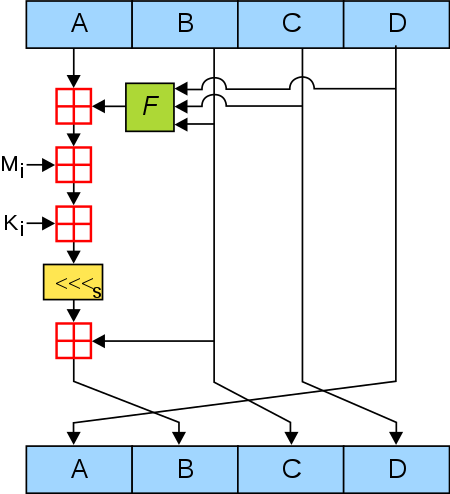
\includegraphics[scale=0.5]{imagenes/md5.png} 
	\caption{Esquema de los pasos seguidos en MD5 \cite{fotosmd5}.}
\end{figure}

\subsection{SHA-0}
SHA-0 es una función hash que apareció publicado en el Federal Information Processing Standard (FIPS-180) por el NIST en 1993 \cite{Penard2008}. Está basado en \emph{MD4} y \emph{MD5}. El algoritmo transforma un mensaje de cualquier tamaño hasta $2^{64}$ bits y los transforma en hashes de 160 bits.\\
El funcionamiento de SHA-0 es el siguiente \cite{sha0}:
\begin{enumerate}
	\item Al igual que en MD5, el mensaje se rellena con un único bit '1' seguido de 0-511 bits '0'. A continuación se añade una representación de 64 bits de la longitud del mensaje donde el número de ceros es elegido para asegurar que la longitud total del mensaje es un múltiplo de 512 bits. El mensaje se divide en bloques de 512 bits: $M_1,...,M_n$.
	\item Para la primera iteración se utiliza un buffer predefinido:
	$$
		h_0=(67452301_x, EFCDAB89_x, 98BADCFE_x, 10325476_x, C3D2E1F0_x).
	$$
	\item Cada bloque $M_j$ es pasado por la función de compresión junto con el valor actual de $h_{j-1}$, la salida es el nuevo valor de $h_j$, la operación se puede resumir en:
	$$
		h_j=compresión(M_j,h_{j-1}).
	$$
	\item $h_n$ es la salida de la función hash.
\end{enumerate}
Los pasos seguidos en la función de compresión son:
\begin{enumerate}
	\item Se divide el bloque $M_j$ de 512 bits en bloques 16 bloques de 32 bits $W_0,W_1,...,W_{15}$. 
	\item Se expanden los 16 bloques de 32 bits en 80 bloques a partir de la siguiente ecuación en recurrencias:
	$$
		W_i=W_{i-3}\oplus W_{i-8}\oplus W_{i-14}\oplus W_{i-16},\; i=16,...,79.
	$$
	Esta expansión se nota como exp(.).
	\item Divide $h_{j-1}$ en 5 registros \emph{A, B, C, D} y \emph{E} como:
	$$
		h_{j-1} = (A_0, B_0, C_0, D_0, E_0).
	$$
	\item Para $i=0,...,79$ hacemos:
	$$
		A_{i+1}=(A_i\lll5)+f_i(B_i,C_i,D_i)+E_i+K_i) \mod 2^{32},
	$$
	$$
		B_{i+1}=A_i,\: C_{i+1}=(B_i\lll30),\: D_{i+1}=C_i,\: E_{i+1}=D_i.
	$$
	Donde las funciones y las constantes están definidas en la tabla \ref{tablasha0}.
	\item La salida de la función sería:
	$$
		h_n=(A_0+A_{80}, B_0+B_{80}, C_0+C_{80}, D_0+D_{80}, E_0+E_{80}).
	$$
\end{enumerate}

\begin{table}[H]
	\begin{center}
		\begin{tabular}{| l | l | l |}
				\hline
				Rondas & $f_i(B,C,D)$ & $K_i$\\ \hline
				$0\leq i\leq 19$ & $BC\vee BD$ & $5AD9EBA1_x$\\ \hline
				$20\leq i\leq 39$ & $B\oplus C\oplus D$ & $6ED9EBA1_x$\\ \hline
				$40\leq i\leq 59$ & $BC\vee BD\vee CD$ & $8F1BBCDC_x$\\ \hline
				$60\leq i\leq 79$ & $B\oplus C\oplus D$ & $CA62C1D6_x$\\ \hline
		\end{tabular}
		\caption{Funciones y constantes usadas en la función de compresión de SHA-0 \cite{sha0}.}
	\label{tablasha0}
	\end{center}
\end{table}

\subsection{SHA-1}
La función SHA-1 es una función hash diseñada en 1995 por la \emph{National Security Agency} (NSA) dado que que se encontró varias colisiones y vulnerabilidades en la función SHA-0 \cite{Penard2008}.\\
Su funcionamiento es muy similar al de la función SHA-0 variando en las funciones y variables usadas en las distintas rondas de la función de compresión. En la tabla \ref{tablasha1} se pueden ver los nuevos valores utilizados.\\
\begin{table}[htb]
	\begin{center}
		\begin{tabular}{| l | l | l |}
				\hline
				Rondas & $f_i(B,C,D)$ & $K_i$\\ \hline
				$0\leq i\leq 19$ & $(B\wedge C)\oplus (\overline{B}\wedge D)$ & $5A827999_x$\\ \hline
				$20\leq i\leq 39$ & $B\oplus C\oplus D$ & $6ED6EBA1_x$\\ \hline
				$40\leq i\leq 59$ & $(B\wedge C)\oplus (B\wedge D) \oplus (C\wedge D)$ & $8FABBCDC_x$\\ \hline
				$60\leq i\leq 79$ & $B\oplus C\oplus D$ & $CA62C1D6_x$\\ \hline
		\end{tabular}
		\caption{Funciones y constantes usadas en la función de compresión de SHA-1 \cite{sha1}.}
		\label{tablasha1}
	\end{center}
\end{table}

En siguiente imagen se puede observar un esquema del proceso para obtener un el hash seguido por las funciones  SHA-0 y SHA-1 donde \textbf{F} será la función de compresión.
\begin{figure}[htb]
	\centering
	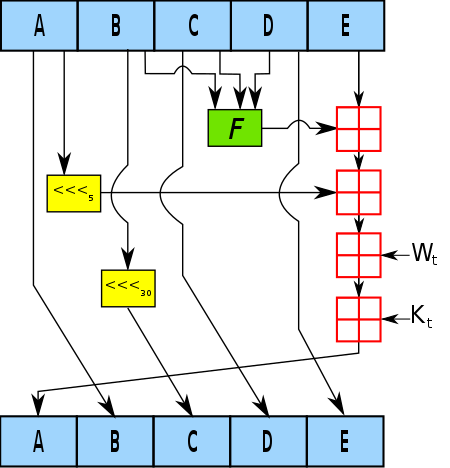
\includegraphics[scale=0.5]{imagenes/sha0-1.png} 
	\caption{Esquema de los pasos seguidos en SHA-0 y SHA-1 \cite{fotosha10}.}
\end{figure}

\subsection{SHA-256}
La función SHA-256 pertenece a la familia SHA-2 que es un conjunto de funciones hash diseñadas por la NSA en 2001 \cite{Penard2008}. Esta familia está compuesta por las funciones SHA-224, SHA-256, SHA-384 y SHA-512 donde el número del final indica el tamaño de bloque en el que se dividirá el mensaje. Nos centraremos en la función SHA-256 que como he comentado anteriormente es la que se utiliza en las aplicaciones de mensajería actualmente.\\
El funcionamiento de las función es el siguiente\cite{Function2016}:\\
\begin{enumerate}
	\item Al igual que en SHA-0 y SHA-1 se rellena el mensaje de la misma manera y se fragmenta en bloques de 512 bits: $M_1,...,M_n$.
	\item Para la primera iteración se utiliza un buffer predefinido:
	$$
		h_0=(H_1, H_2, H_3, H_4, H_5, H_6, H_7, H_8),
	$$
	donde:\\
	$H_1=6A09E776$\\
	$H_2=BB67AE85$\\
	$H_3=3C6EF372$\\
	$H_4=A54FF53A$\\
	$H_5=510E527F$\\
	$H_6=9B05688C$\\
	$H_7=1F83D9AB$\\
	$H_8=5BE0CD19$\\
	\item Cada bloque $M_j$ es pasado por la función de compresión junto con el valor actual de $h_{j-1}$, la salida es el nuevo valor de $h_j$, la operación se puede resumir en:
	$$
		h_j=compresión(M_j,h_{j-1}).
	$$
	\item $h_n$ es la salida de la función hash.
\end{enumerate}
Los pasos seguidos en la función de compresión son:
\begin{enumerate}
	\item Se divide el bloque $M_j$ de 512 bits en bloques 16 bloques de 32 bits $W_0,W_1,...,W_{15}$. 
	\item Se expanden los 16 bloques de 32 bits en 63 bloques a partir de la siguiente ecuación en recurrencias:
	$$
		W_i=\sigma_1(W_{j-2})+W_{j-7}+\sigma_0(W_{j-16}),\; i \in \{16...63\}.
	$$
	\item Divide $h_{j-1}$ en \emph{A, B, C, D, E, F, G} y \emph{H} como:
	$$
		h_{j-1} = (A_0, B_0, C_0, D_0, E_0, F_0, G_0, H_0).
	$$
	\item Para $i=0,...,63$ hacemos:
	$$
		A_{i+1}=H_i+\Sigma_1(E_i)+Ch(E_i,F_i,G_i)+K_j+W_j+\Sigma_0(A_i)+Maj(A_i,B_i,C_i),
	$$
	$$
		B_{i+1}=A_i,\: C_{i+1}=B_i,\: D_{i+1}=C_i,\: F_{i+1}=E_i\: G_{i+1}=F_i,\: H_{i+1}=G_i,
	$$
	$$
		E_{i+1}=D_i+H_i+\Sigma_1(E_i)+Ch(E_i,F_i,G_i)+K_j+W_j.
	$$
	Donde las funciones y las constantes están definidas en la tabla \ref{tablasha0}.
	\item La salida de la función sería:
	$$
		h_j=(A_0+A_{63}, B_0+B_{63}, C_0+C_{63}, D_0+D_{63}, E_0+E_{63}, F_0+F_{63}, G_0+G_{63}, H_0+H_{63}).
	$$
\end{enumerate}
Donde tenemos que:
$$
	Ch(x,y,z) = (x\wedge y)\oplus (\overline{x}\wedge z),
$$
$$
	Maj(x,y,z) = (x\wedge y)\oplus (x\wedge z)\oplus (y\wedge z),
$$
$$
	\Sigma_0(x) = (x\ggg2)\oplus (x\ggg13)\oplus (x\ggg22),
$$
$$
	\Sigma_1(x) = (x\ggg6)\oplus (x\ggg11)\oplus (x\ggg25),
$$
$$
	\sigma_0(x) = (x\ggg7)\oplus (x\ggg18)\oplus (x\lll3),
$$
$$
	\sigma_1(x) = (x\ggg17)\oplus (x\ggg19)\oplus (x\lll10).
$$

%\newpage
En la siguiente imagen podemos ver un esquema de los pasos seguidos en las funciones SHA-2.\\
\begin{figure}[htb]
	\centering
	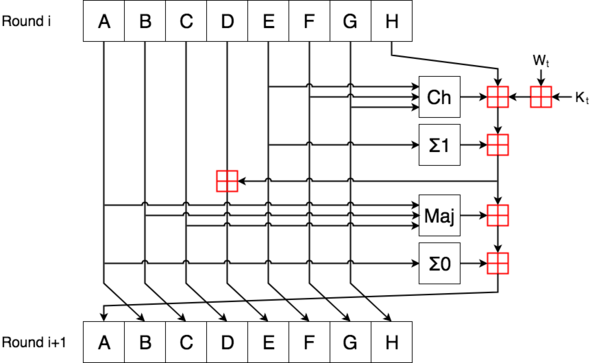
\includegraphics[scale=0.5]{imagenes/sha2.png} 
	\caption{Esquema de los pasos seguidos en las funciones de la familia SHA-2 \cite{sha2wikipedia}.}
\end{figure}

Con esto concluye el capítulo en el cual se han introducido todas las herramientas necesarias para entender los criptosistemas de las aplicaciones de mensajería. En el próximo capítulo procederé a explicar los criptosistemas utilizados en algunas de las aplicaciones de mensajería más populares.
